% Template for ICIP-2014 paper; to be used with:
%          spconf.sty  - ICASSP/ICIP LaTeX style file, and
%          IEEEbib.bst - IEEE bibliography style file.
% --------------------------------------------------------------------------
\documentclass{article}
\usepackage{spconf,amsmath,graphicx}
\usepackage{multirow}
\usepackage{algorithm}
\usepackage{algpseudocode}
\usepackage{graphicx}									
\usepackage{subfigure}


\renewcommand{\algorithmicrequire}{\textbf{Input:}} % Use Input in the format of Algorithm
\renewcommand{\algorithmicensure}{\textbf{Output:}} % Use Output in the format of Algorithm



% Example definitions.
% --------------------
\def\x{{\mathbf x}}
\def\L{{\cal L}}

% Title.
% ------
\title{Discrimination of ADHD children based on Deep Bayesian Network}
%
% Single address.
% ---------------
\name{A. Junyu Hao, B. Lianghua He \thanks{Thanks to National Natural Sciences Foundation of China.(No.61272267, 61270220, 51075306,61273261)}}
\address{Tongji University,
Department of Computer Science and Technology\\}
%
% For example:
% ------------
%\address{School\\
%	Department\\
%	Address}
%
% Two addresses (uncomment and modify for two-address case).
% ----------------------------------------------------------
%\twoauthors
%  {A. Author-one, B. Author-two\sthanks{Thanks to XYZ agency for funding.}}
%	{School A-B\\
%	Department A-B\\
%	Address A-B}
%  {C. Author-three, D. Author-four\sthanks{The fourth author performed the work
%	while at ...}}
%	{School C-D\\
%	Department C-D\\
%	Address C-D}
%
\begin{document}
%\ninept
%
\maketitle
%
\begin{abstract}
Attention deficit hyperactivity disorder (ADHD) is a threat for the public health all the time, so the effective discrimination of it is significant and meaningful. In current research, Functional Magnetic Resonance Imaging (fMRI) data has become a popular tool for the analysis of ADHD. In this paper, we introduce the Deep Bayesian Network, a combination of Deep Belief Network and Bayesian Network, to classify the ADHD children from the normal. In Deep Bayesian Network, The Deep Belief Network is applied to  normalize and reduce dimension of the fMRI data in every brodmann area. And the Bayesian Network is used to extract the feature of relationships between several well-performed brain areas by structure learning. According to the information of structure and probability in Bayesian Network, we predicted the subjects as control,combined ,inattentive or hyperactive using SVM classifier. The final results perform better than using single Deep Belief Network and the best results in ADHD-200 competition. 

\end{abstract}
%
\begin{keywords}
ADHD, Deep Learning, Bayesian Network, SVM, Deep Belief Network
\end{keywords}
%
\section{Introduction}
\label{sec:intro}

Attention deficit hyperactivity disorder (ADHD) is among the most common psychiatric disorders of childhood that persists into adulthood in the majority of cases\cite{1}. According to American Psychiatric Association’s Diagnostic and Statistical Manual, the prevalence of ADHD in the whole world is approximately 5\%, especially in the United States the prevalence among 8 to 15-years-olds reaches to 8.7\% during the past years. Therefore, the methods of diagnosing the ADHD are in urgent need.
 
 
 
As an excellent method of measuring brain activation, fMRI
signals are studied to classify ADHD. Shengfu Liang et al.\cite{3} utilizes the LDA classifier to discriminate ADHD by analyzing the rs-fMRI data, and the average accuracy of distinguishing normal and ADHD children reaches 80.08\% through 50 times of 2-fold validation. Xunheng Wang\cite{4} applies Kernel Principal Component Analysis (KPCA) method based on connectivity matrix of each functional meaningful brain region to find the abnormal pattern of ADHD. Then Support Vector Machine (SVM) as a classifier increases the accuracy rate to 81\% using a leave-one-out cross validation. In the global ADHD-200 competition, Eloyan A et al.\cite{6} has achieved relatively better scores by using rs-fMRI based on decomposition of CUR along with gradient boosting. In this paper, three datasets from ADHD-200 competition are applied to discriminate ADHD.

\begin{figure*}[ht]
\begin{center}
%\fbox{\rule{0pt}{2in} \rule{0.9\linewidth}{0pt}}
   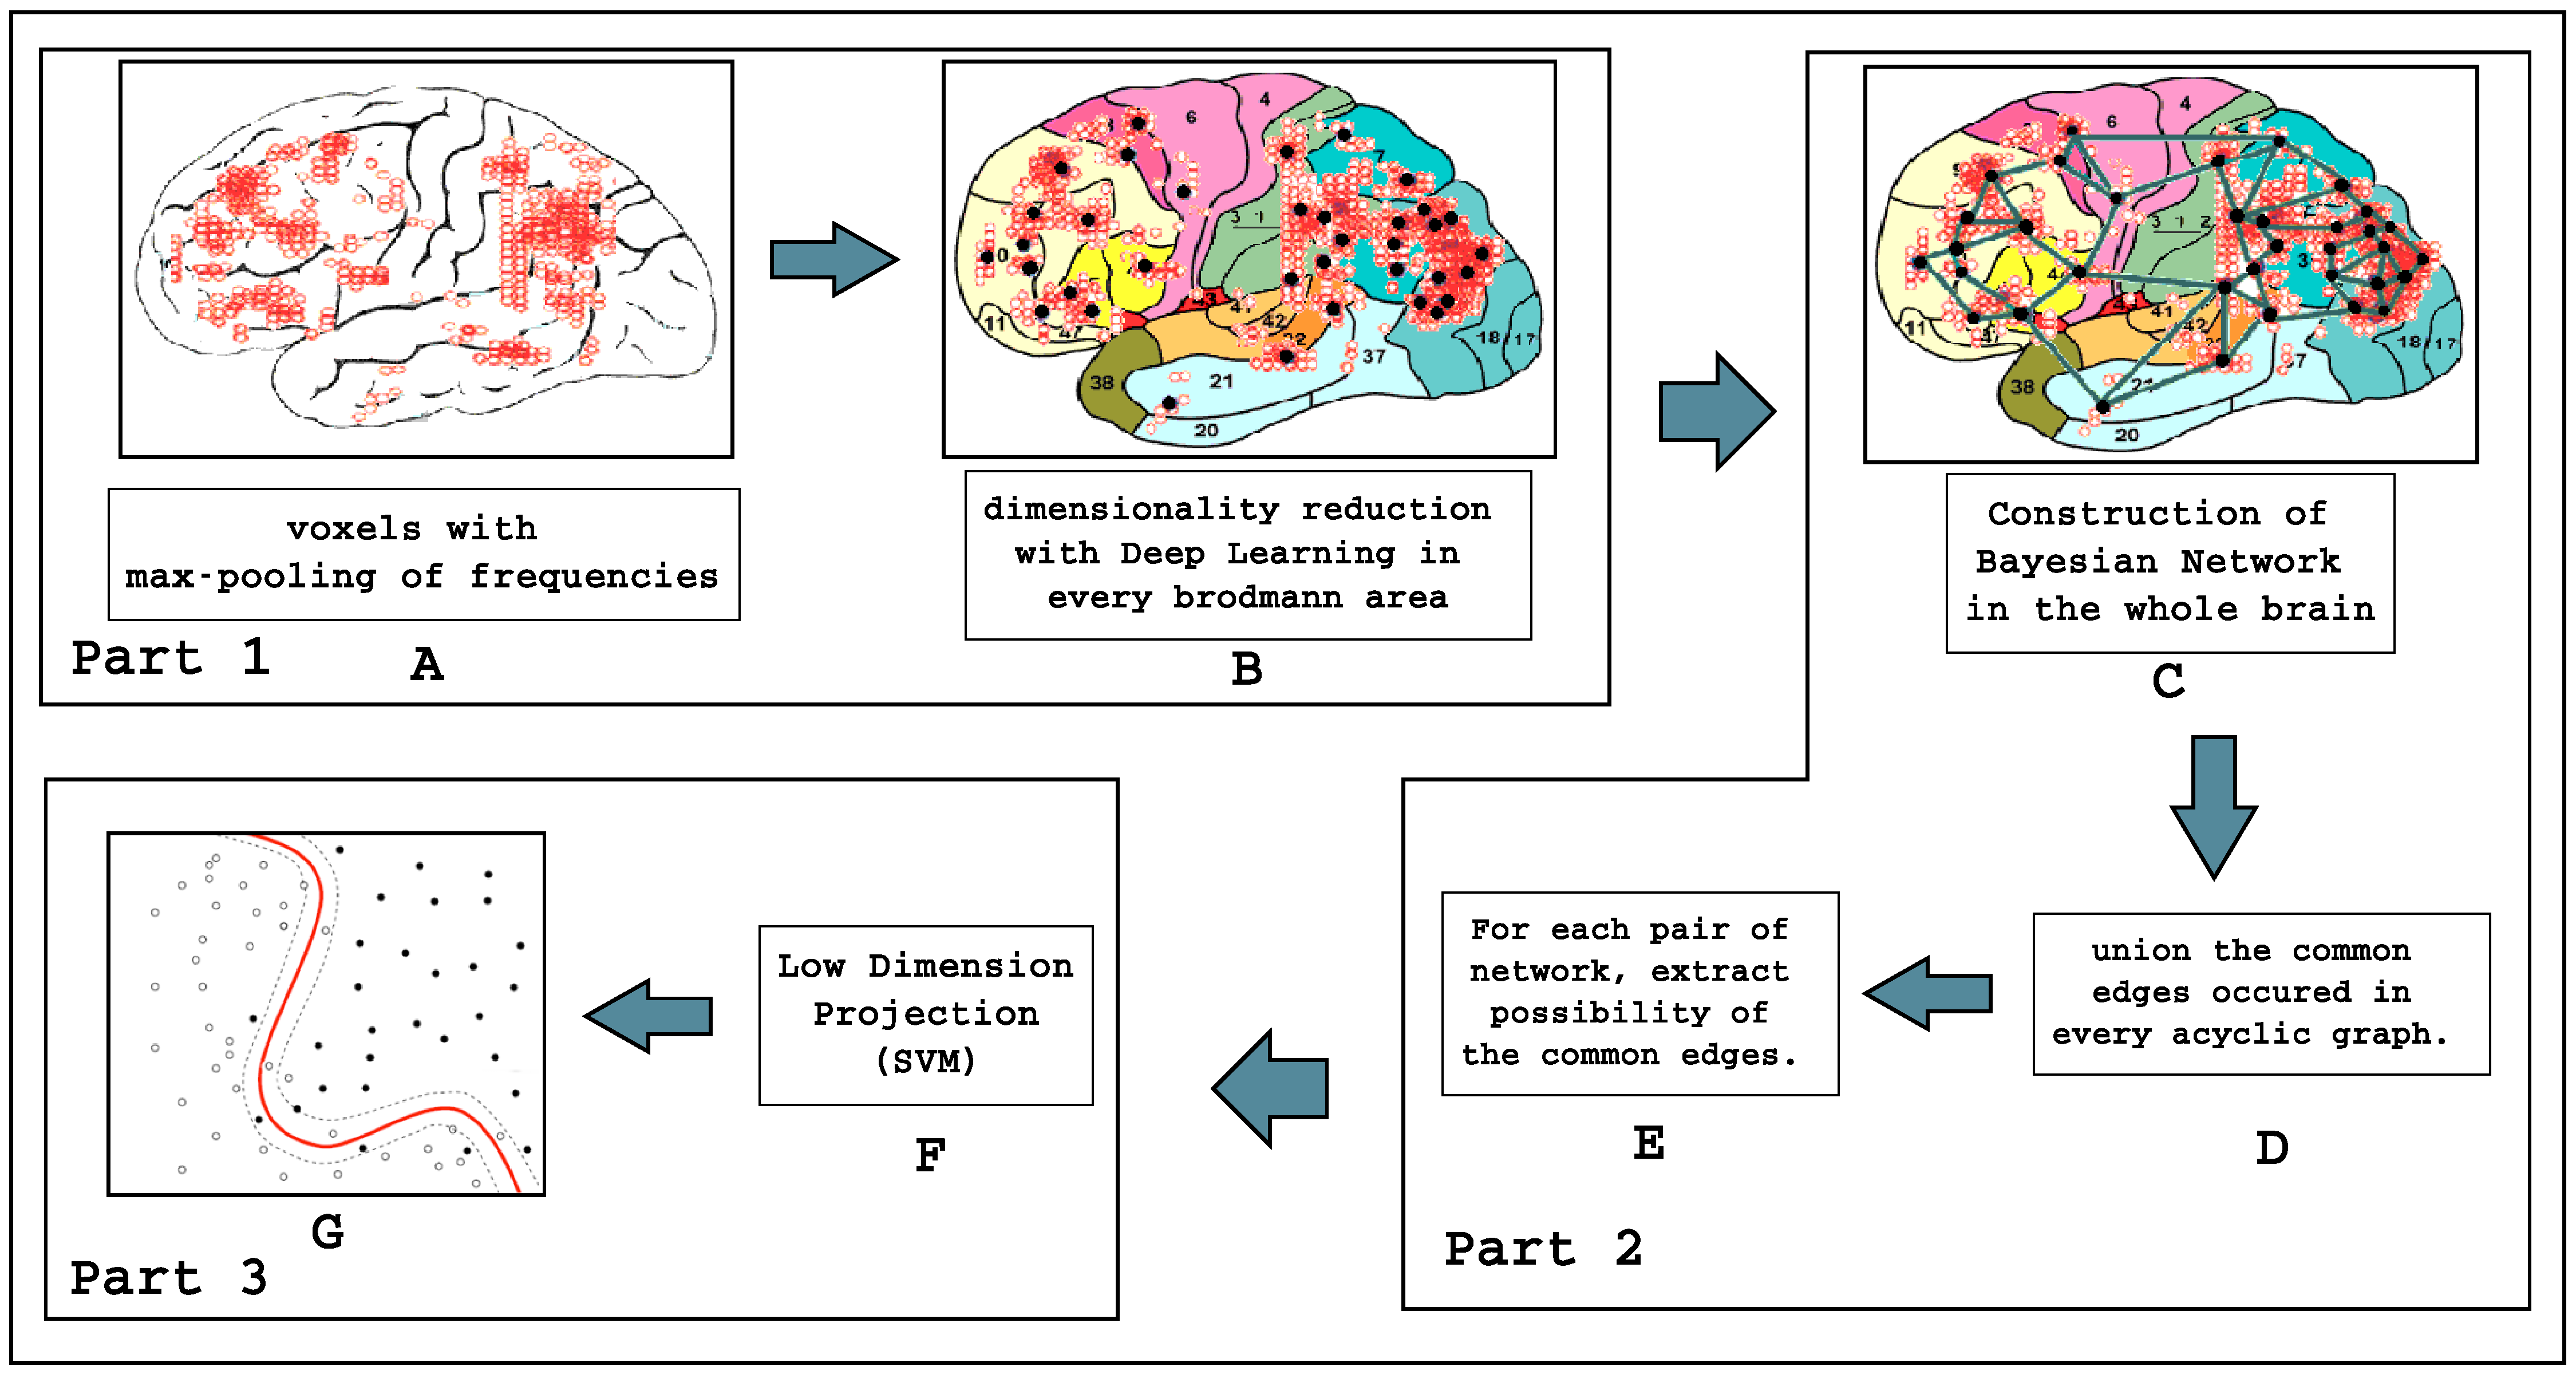
\includegraphics[width=460pt, height=115pt]{Figures/overviews.eps}
\end{center}
   \caption{The procedure of Deep Bayesian Network}
\label{fig:overview}
\end{figure*}


However, it will encounter a serious problem during analyzing the ADHD with fMRI data, which are the mass of data and data redundancy. Therefore, dimensionality reduction is essential. Although there are many dimensionality reduction methods proposed, but they only take mathematical requirements into consideration, rather than physical requirements. Luckily, Geoffrey E.Hinton et al.\cite{8} derives a fast, greedy algorithm that can learn deep, directed belief networks one layer at a time, provided the top two layers form an undirected associative memory by using complementary prior.  Because of the good performance in dimensionality reduction currently, Deep Learning has been applied for many areas including image processing\cite{8}, audio classification\cite{9}, natural language processing\cite{12} and so on.


Due to the cause in ADHD cases is unknown, the relationships between different areas should be token into consideration rather than analysis the brain area separately, which meets the requirements of Bayesian network. It is a graphical model that can encode probabilistic relationships among variables of interest. On the one hand, the model can be used to learn causal relationships and gain understanding about a problem domain. For example, in bioinformatics Bayesian network has been used for the interpretation and discovery of gene regulatory pathways\cite{14}. On the other hand, it is an ideal representation for combining prior knowledge and data. Based on these, Bayesian network has been used in information retrieval\cite{15}, natural language processing\cite{16} and so on.

 
Figure 1 shows the framework of proposed method. It can be seen that there are totally four steps. The first step is that pre-process the
voxels with max-pooling of frequencies(\textbf{A} in Fig.\ref{fig:overview}). Then, Deep Belief Network is used to reduce dimensionality of data in every brodmann area(\textbf{B} in Fig.\ref{fig:overview}), which reconstructs the different number of voxels in every areas into the same number of features, and the Bayesian network can extract the relationships with the normalized fMRI data(\textbf{C-E} in Fig.\ref{fig:overview}). These two steps are the highlights of Deep Bayesian Network. Finally, using SVM as a classifier to discriminate the ADHD children from normal(\textbf{F-G} in Fig.\ref{fig:overview}).





\section{METHOD}
The proposed method, Deep Bayesian Network, can be divided into two main parts such as Deep Belief Network for  normalization and Dimensionality reduction(Part 1 in Fig.\ref{fig:overview}), Bayesian Network construction for feature extraction(Part 2 in Fig.\ref{fig:overview}). The following sections describe each parts in details. Finally, the SVM is used as a classifier(Part 3 in Fig.\ref{fig:overview}).

\subsection{Deep Belief Network}
Deep Belief Network is made of a stack of
restricted Boltzmann machines(RBM)\cite{13}. It is a two-layer, undirected, bipartite graphical model including visible units and hidden units. The weights $W$ and biases $a,b$ of the RBM determine the energy of
a joint configuration of the hidden and visible units $E(v,h)$,
\begin{equation}
E(v,h;\theta) = -\sum_{i=1}^V \sum_{j=1}^H v_ih_jw_{ij} - \sum_{i=1}^V b_iv_i - \sum_{j=1}^H a_jh_j
\end{equation}
with model parameters $\theta = \{W,b,a\}$ and $v_i,h_j \in \{0,1\}$. 

In general Boltzmann machines, the probability distributions are defined in terms of the energy function $p(v,h) = \frac{1}{z} \exp ( -E(v,h) )$,
where $z$ is defined as the sum of $\exp ( -E(v,h) )$.
Based on $p(v,h)$, the conditional probability of $v$ given $h$ and of $h$ given $v$.

By now, the pre-train of RBM network has mapped the input data into different feature space and kept much feature information. So back propagation is needed to spread the error message to each level of RBM from the top to down. Following the gradient of the log likelihood $\log P(v)$, we obtain the update rule for the weights as,
\begin{equation}
\Delta w_{ij} = \epsilon (<v_i,h_j>_{data} - <v_i,h_j>_{recon})
\end{equation}
Where $\epsilon$ is the learning rate and the angle brackets manifests the expectations relative to the distribution specified in the subscript. 


\subsection{Bayesian Network}
A Bayesian network $B=<N,A,\Theta>$ is a directed acyclic graph (DAG) $<N,A>$ with a conditional probability table (CPT) for each node, collectively represented by $\Theta$. Each node $n \in N$ represents a domain variable $x_i$, and each arc $a \in A$ between nodes represents a probabilistic dependency $p(x_i|x_j)$. The joint probability $p(X)$ can be calculated as follows:
\begin{equation}
p(X) =\prod_{i=1}^m p(x_i |\pi_i))
\end{equation}
where $\pi_i$ denotes the parent $i=1,\cdots,m$ nodes of $x_i$.
There are two major tasks in learning a BN: structure learning and parameters learning. This paper mainly uses the structure to extract the information, so we apply  Max-Min Hill Climbing (MMHC) algorithm to learn structure efficiently, which is most suitable to the brain areas.





\subsection{The Construction of Deep Bayesian Network}
\subsubsection{Deep Feature Extraction}
In this paper, the original fMRI data $D$ is a time series, so it can not be used as the input for deep belief network in every brodmann area. The frequency information can be used as the characteristics of each voxel by the study in our research group. So the input of Deep Belief Network $X$ is pre-processed by realign, slice time, co-register, normalize,smooth which are described in this paper\cite{18} in detail after fast Fourier transform algorithm (FFT). 
\begin{equation}
X_f = fft(D) 
\end{equation}
To construct the Deep Belief Network, the forward calculation and backward propagation are needed in every layer.
\begin{eqnarray}
[\theta,X] &=& RBN(X)   \\
\theta  &=& backprop(\theta,X)
\end{eqnarray}
The pseudo-code for application of Deep Belief Network on ADHD data can be seen as following Algorithm \ref{code:DBN} .
\begin{algorithm}[h]
\caption{Deep Feature Extraction}
\label{code:DBN}
\begin{algorithmic}[1]
\Require
original fMRI data $D$

\State Get frequencies in every voxel $X_f$
\[ X_f \gets fft(D)\]
\State Pre-process frequency information: $X \gets prepro(X_f)$ 
\For{$k \gets 1, 3$} 
\State train the weights $\theta=[w,a,b]$ of single rbm
\[
[\theta,X]\gets RBN(X)
\]
\EndFor
\State Adjust weights with Backpropagation
\[
\theta \gets backprop(\theta,X)
\]
\State Reduce dimensionality:  $Y \gets DBN(\theta,X)$ 
\Ensure
dimensionality-reduced data $Y$
\end{algorithmic}
\end{algorithm}


\subsubsection{Structure Learning of Deep Bayesian Network}
Duo to the reason of ADHD is unknown, it is meaningful to analysis the
dimensionality-reduced data $Y$ and sample label $L$ in the
whole brain with Bayesian Network. First, filter the data $Y$ to wipe out the noise. Second, the MMHC algorithm can speed up the structure of Bayesian network, but it needs the limited parent nodes of each node. So the dependent nodes $I$ are computed by conditional independence testing in filtered data $Y_f$.
\begin{equation}
I = indep(Y_f)
\end{equation}
Third, we union the limited parent nodes $U$ and use it to learn the structure of all data including training data and testing data. By this, we can get a DAG $G$ and a table $P$ including the information of probability of edge shown in equation below.
\begin{equation}
[G,P] = BN(U,Y_f)
\end{equation}
Forth, the probability of each edge in Bayesian network will be extracted out and viewed as feature $F$ of ADHD children and normal children. Finally, SVM will be acted as classifier to train the training samples and classify the testing samples, which will get the classified label of testing sample $C$. The accuracy $T$ can be computed by predicted labels $L$ and true labels $Y$. The pseudo-code for application of BN on ADHD data can be seen as following Algorithm \ref{code:BN}.  
\begin{algorithm}[h]
\caption{Structure Learning of Deep Bayesian Network}
\label{code:BN}
\begin{algorithmic}[1]
\Require
dimensionality-reduced data $Y$, labels of data $L$

\State Filter the data: $X_{f} \gets filter(Y)$ 
\State Test Conditional independence
\[
I \gets indep(X_{f})
\] 
\State union the parent's limitation: $U \gets union(I)$
\State Learning structure of Bayesian Network
\[ [G,P] \gets BN(U,Y_f)
\]
\State Extract feature: $F \gets extract(G,P)$
\State Classify the features: $C \gets svm(F,L)$ 
\State Computer accuracy: $T \gets com(L,C)$ 
\Ensure
accuracy of discrimination $T$
\end{algorithmic}
\end{algorithm}



\section{EXPERIMENTS AND RESULTS}
\subsection{Data}
The data used in this paper can be downloaded from the ADHD-200 Global Competition website. DBN and BN model is built upon the ADHD dataset for NYU, Peking-1 and KKI respectively.


For NYU, the training subjects are 216, and testing subjects are 41; for Peking-1 dataset, the training subjects are 85, and testing subjects are 50; and for KKI the training subjects and testing subjects are 83 and 11 respectively. The detail information for the subjecets is shown in Table 1.


\begin{table}[h]
\label{tab:Information}
\caption{Demographic Information of three Datasets}
\begin{center}
\begin{tabular}{|c|c|c|c|c|c|c|}
\hline
\multirow{3}{*}{type}	& \multicolumn{2}{c|}{NYU} & \multicolumn{2}{c|}{Peking-1} & \multicolumn{2}{c|}{KKI} \\
\cline{2-7}\rule{0pt}{5pt}
					 	& train &  test  & train	& test 	& train & test  \\
						& 216	& 41	  &    85   &   50  &   83   &   11 \\ [2pt]
\hline \rule{0pt}{12pt}
control					& 98	    & 12    &    61   &    27 &   61    &   8 \\
combined					& 73		& 22   &    7    &    9  &   16    &   3 \\
inattentive				& 2		& 0    &    0    &    1  &   5     &   0 \\
hyperactive				& 43		& 7    &    17   &    13 &   1    &   0 \\[2pt]
\hline
\end{tabular}
\end{center}
\end{table}



\subsection{The Experiment of Parameter Design}
To construct a Deep Bayesian Network, we must set up the number of selected areas. If the value of number is small, Bayesian network will not extract the enough information of relationships between brain areas. If the value of number is too large, the probability that the unrelated brain areas will be chose as a node will get higher, which has a side effect on the final classification. In addition,  with the increase of the variables, the search space of network structure will present exponentially. So the experiment of parameter designing is significant.
\subsubsection{Parameter Design in NYU dataset}
As NYU dataset in the ADHD-200 competition achieved the lowest discrimination results, Deep Belief Network is particularly tested on the NYU dataset of 48 areas and softmax as a classifier generates the accuracies of different brain areas,which is convenient for the choice of node in the Bayesian network. The results of 41 regions are shown in Figure~\ref{fig:NYU}.
\begin{figure}[ht]
\begin{center}
\subfigure[Accuracy of NYU in 48 Areas]{
   \label{fig:NYU}
   \includegraphics[width=0.8\linewidth]{Figures/NYU.png}}
\subfigure[Accuracy in Different Number of Brain Areas]{
   \label{fig:BN}   
   \includegraphics[width=0.9\linewidth]{Figures/BN.png}}
   \caption{Parameter Design in NYU dataset}
\end{center}
\end{figure}


From Figure~\ref{fig:NYU}, we can see that different brain areas have different performance of discrimination. The areas of 10, 18, 30, 9, 11, 19, 34, 32, 8, 17, 2, 28, 3, 1, 7, 23, 25, 41 perform well. According to brodmann definition, it is clear that prefrontal cortex(9,10,25), visual cortex(8,17,18,19), somatosensory cortex(1,2,3,7) and cingulate cortex(23,30,32) is related to the ADHD closely. Therefore, they are selected as the input of Bayesian Network.  The Figure ~\ref{fig:BN} shows that the accuracy of discriminate fluctuate a little from 10 to 18, but it reaches the peak when the number of brain areas is equal 15. So we will choose 15 brain areas in the front to construct the Bayesian network. Besides, using the relationships between brain areas to discriminate ADHD is better than using information in single brain area and the best result in  ADHD-200 competition.



%\begin{figure} 
%  \centering 
%  \begin{minipage}[t]{.25\textwidth} 
%    \begin{flushleft}
%    \includegraphics[width=0.7\linewidth]{Figures/Datasets.eps}
%    \caption{Performance in Different Datasets} 
%    \label{fig:dataset}
%    \end{flushleft}
%  \end{minipage}% 
%  \begin{minipage}[t]{.25\textwidth} 
%    \begin{flushright}
%    \includegraphics[width=0.7\linewidth]{Figures/Number.eps}
%   	\caption{Performance in Different Number of training samples}
%   	\label{fig:Number} 
%    \end{flushright}
%    
%  \end{minipage}% 
%\end{figure}




\subsection{Performances on NYU, Peking-1 and KKI dataset}
The experiments are also excuted on the NYU, Peking-1 and KKI dataset. The results released by ADHD-200 competition are 35.19\% for NYU, 51.05\% for Peking-1 and 61.90\% for KKI respectively. The prediction accuracies of Attributed graph distance\cite{19} (AGD) are none, 58.82\%,54.55\%. The Deep Bayesian Network  gains a higher prediction accuracies than Deep Belief Network single, which are 48.78\% for NYU, 54.00\% for Peking-1 and 72.72\% for KKI. The details show in Figure ~\ref{fig:dataset}.
\begin{figure}[ht]
\begin{center}
%\fbox{\rule{0pt}{2in} \rule{0.9\linewidth}{0pt}}
   \includegraphics[width=0.8\linewidth]{Figures/Datasets.png}
\end{center}
   \caption{Performance in Different Datasets}
\label{fig:dataset}
\end{figure}


From this chart, we can see that Deep Bayesian Network improves the prediction accuracies  in these three datasets  compared with the results of ADHD-200 competition. Besides, the increase of accuracy is the highest in the NYU dataset than other two datasets. The different number of training samples have a big effect on the accuracy. This effect is shown in Figure ~\ref{fig:Number}.
\begin{figure}[ht]
\begin{center}
%\fbox{\rule{0pt}{2in} \rule{0.9\linewidth}{0pt}}
   \includegraphics[width=0.8\linewidth]{Figures/Number.png}
\end{center}
   \caption{Performance in Different Number of training samples}
\label{fig:Number}
\end{figure}



Considering that discriminating the ADHD is important and meaningful, here we take the prediction accuracy of the method along with the specificity and sensitivity values into consideration. The detail information is shown in Tab 2.

%NYU			&  -		&   -	 &  - &  64.65	&  68.77 & 43.89 \\[2pt]
%Peking-1		& 58.82		&  92.59 	& 20.83 & 66.32 & 87.71 &22.88\\[2pt]
%KKI			& 54.55		& 62.50	& 33.33 & 58.96  & 82.98  & 55.56\\[2pt]


\begin{table}[h]
\label{tab:2}
\caption{The Detail information in Different Datasets}
\begin{center}
\begin{tabular}{cccc}
\hline

Dataset  	&   Accuracy  	&	Specificity  &	Sensitivity \\
\hline
NYU			&  64.7	&  68.8 & 43.9 \\[2pt]
Peking-1		& 66.3 & 87.7 &22.9\\[2pt]
KKI			& 59.0  & 83.0  & 55.6\\[2pt]
\hline
\end{tabular}
\end{center}
\end{table}







%------------------------------------------------------------------------
\section{CONCLUSION}
In this paper, a novel method called Deep Bayesian Network, is proposed to classify fMRI ADHD image data. Because of the combination Deep Belief network and Bayeisan network, Deep Bayesian Network can compute relationships among brodmann brain areas more effectively. A series of experimental results also prove that Deep Bayesian network  improves the classification performatnce of ADHD greatly comparing with the ADHD-200 competition resutls. 





% References should be produced using the bibtex program from suitable
% BiBTeX files (here: refs). The IEEEbib.bst bibliography
% style file from IEEE produces unsorted bibliography list.
% -------------------------------------------------------------------------
\bibliographystyle{IEEEbib}
\bibliography{refs}

\end{document}
